\documentclass{article}
\author{Stefan Countryman}
\usepackage[utf8]{inputenc}
\usepackage[colorlinks, urlcolor=cyan]{hyperref}
% display code; from: https://stackoverflow.com/questions/3175105/writing-code-in-latex-document
\usepackage{listings}
\usepackage{color}
\usepackage{geometry}
\usepackage{graphicx}
\usepackage{wrapfig}

\definecolor{dkgreen}{rgb}{0,0.6,0}
\definecolor{gray}{rgb}{0.5,0.5,0.5}
\definecolor{mauve}{rgb}{0.58,0,0.82}

\lstset{frame=tb,
  aboveskip=3mm,
  belowskip=3mm,
  showstringspaces=false,
  columns=flexible,
  basicstyle={\small\ttfamily},
  numbers=none,
  numberstyle=\tiny\color{gray},
  keywordstyle=\color{blue},
  commentstyle=\color{dkgreen},
  stringstyle=\color{mauve},
  breaklines=true,
  breakatwhitespace=true,
  tabsize=3
}

\title{LIGO Site Visit Checklist}

\definecolor{todo}{RGB}{170, 86, 73}        % light rust
\newcommand*{\TODO}{\textcolor{todo}}

\begin{document}
\maketitle

\begin{abstract}
\emph{This document contains a generic timing system to-do list for a visit to one of the LIGO sites. You should make a copy of this tex file and add any extra items for a specific trip along with a descriptive abstract. As you work on things, you should take notes in this tex file and expand it out so that it eventually becomes a report. If you're working on things besides timing, give them their own sections. Put supporting documents in the appendix. You can mark items that need to be done with a \texttt{\\TODO} command in the \texttt{tex} file; items marked this way are \TODO{marked in a light rust color}.}
\end{abstract}

\section{Timing}

\TODO{
\subsection{Finish measuring cable lengths/types}
}
Might need to do 
\href{https://en.wikipedia.org/wiki/Time-domain_reflectometer}{TDR})
to get remaining cable lengths.
\footnote{
    Cable length Google spreadsheet \href{https://docs.google.com/spreadsheets/d/1cjpBtpd4oPAfjNjBhE3RXxSx3ma3oopqLLZFMjEjc0w/edit\#gid=0}{here}, based on \href{https://docs.google.com/spreadsheets/d/1AfZ9m7Qetefmtr-PnHNARC14OWaPfn0z5c9GOvcojyA/edit\#gid=0}{LLO Google spreadsheet} (LLO cable measurements copied \hyperref[sec:llocables]{in the appendix}).
}
You can get the cable names by going to the cable locations and looking for little labels attached to the cables. The cable type will be printed directly onto the cables all along their lengths; RG-58 is a common cable type. You'll need to measure the lengths yourself (don't worry about accuracy better than a foot or so overall). The easily-accessible cables have already been measured, hence the possible need for TDR (see notes after table).
Record cable information in Table~\ref{table:lho-cables}.

We won't be able to take measurements on antenna cables; will need to approximate those with Dave and then maybe TDR them in a more painful measurement later (since we would probably need to disconnect the roof antenae). Alternatively, we could estimate the length to within $\pm10$ feet using the design document for the end station along with an understanding of the routing of the cable from the CNS II to the end station roof antenna (Dave Barker knows how this is routed; he drew 
\hyperref[fig:routing]{a cartoon}, but we'll need to bug him for a more precise routing), though this seems like a lot of trouble for an imprecise measurement. aLOG for 1PPS measurements 
\href{https://alog.ligo-wa.caltech.edu/aLOG/index.php?callRep=43185}{here}. See Fig. \ref{fig:rainertdr} for a pic of Rainer performing a TDR measurement.

\textbf{Update:} We will do this next Tuesday (maintenance day). We will start at the end stations because, according to Dave, they have their antennae at the edges (while the corner station has its GPS antennae on the weather station, more than 6 feet from the edge, at least at LHO).

\textbf{Update:} Opened \href{https://services.ligo-la.caltech.edu/LHO/workpermits/view.php?permit_id=8044}{work permit 8044} for this work. We will start by measuring the cable lengths at the end stations since this will not require disconnecting anything related to the Timing \textit{Distribution} System.

\textbf{Update:} Filoberto showed Stef how to use a TDR (fig.~\ref{fig:tdr-tool}) to take measurements (Instructions in fig.~\ref{fig:tdr-dtf-instructions}). We tested it in the EE Shop with a 150ft RG-58C/U cable and a GPS antenna (fig.~\ref{fig:tdr-test}) as proof-of-concept; since we can't remove the GPS Antenna at the rooftop end of the cable without getting up to the roof (which requires harness certification), we wanted to check that a DTF (distance to fault) measurement would work with a GPS antenna terminating the cable.

For the distance measurement, we will be using Distance to Fault (DTF) mode, which will require inputting a rough estimate of the distance to the GPS antenna (overestimating is good since this distance specifies the bounds of our distance search; 200ft is probably a good starting point). 

\begin{itemize}
    \item{\TODO{Get adapters for the GPS antenna cable.}}
    \item{\TODO{Get the Velocity Factor for whatever cable type is used for the GPS antenna.}} If it's LMR-195 Like at Livingston, then the velocity factor will be \href{https://www.pasternack.com/50-ohm-low-loss-flexible-lmr195-pe-jacket-double-shielded-black-lmr-195-p.aspx}{0.8}.
    \item{\TODO{Get screwdriver for removing rack-mounted CNS II clock.}}
    \item{\TODO{Grab the TDR tool}}
    \item{\TODO{Uninstall CNS II from rack and leave with Dave Barker}}
    \begin{itemize}
        \item \TODO{At X End}
        \item \TODO{At Y End}
    \end{itemize}
    \item{\TODO{Perform TDR measurement and record cable type and cable name}}
    \begin{itemize}
        \item \TODO{At X End}
        \item \TODO{At Y End}
    \end{itemize}
\end{itemize}

\begin{center}
  \label{table:lho-cables}
  \begin{tabular}{ | l | l | l | l | }
    \hline
    \textbf{Description}  			& \textbf{Length [ft]} 	& \textbf{Type} 		& \textbf{Cable Name (if applicable)} \\ \hline
    Y-End CNS II 1PPS  				& 29 					& RG-58 				& CDS\_GPS\_COMPARATOR \\ \hline
    X-End CNS II 1PPS				& 29					& RG-58					& CDS\_GPS\_COMPARATOR \\ \hline
    Symmetricom 1PPS to Comparator	& 5 					& RG-58					& SYMMETRICOM\_1PPS \\ \hline
    NTP Server 1PPS to Comparator	& 5 					& RG-58					& C50-005-0025 \\ \hline
    Cs-III 1PPS to Comparator		& 5 					& RG-58					& C50-005-0019 \\ \hline
    Trimble to Master 1PPS cable	& 2 					& RG-58					& \\ \hline
    Timing Master GPS Antenna Cable	&  						& 						& \\ \hline
    Trimble GPS Antenna Cable		&  						& 						& \\ \hline
    Y-End CNS II GPS Antenna Cable	&  						& 						& \\ \hline
    X-End CNS II GPS Antenna Cable	&  						& 						& \\ \hline
    Lightning arrestor to Trimble	&  						& 						& \\ \hline
    Lightning arrestor to Master	&  						& 						& \\
    \hline
  \end{tabular}
\end{center}

\TODO{
\subsection{
    Update or confirm
    \href{https://dcc.ligo.org/LIGO-D1500201}{installed timing map at LHO} (GitHub repo
    \href{https://github.com/stefco/geco_channels}{here}).
}
}
\textbf{Note:} The items below are from the last visit and still need to be done, but you'll need to check the installation \textit{again} to confirm that things have not changed since the last visit in August 2018. 
\begin{itemize}
  \item{\TODO{Remove TCT/TCG from LHO diagrams}}
  \item{\TODO{Add cable lengths to both diagrams}}
  \item{\TODO{Add cable types to both diagrams via legend}}
  \item{\TODO{Add links to 1PPS diagnostic channels}}
  \item{\TODO{Add some photos to LHO and LLO maps}}
  \item{\TODO{Upload saved changes to DCC}}
\end{itemize}

\TODO{
\subsection{Calibrate atomic clock}
}
Download a few months of atomic clock (i.e. Cesium clock) data in order to see if it's drifting significantly. If the clock is drifting quickly away from the actual GPS time, then the Cesium clock must be recalibrated. You can download the Cesium clock data using the \href{https://github.com/stefco/geco_data/blob/master/geco_gwpy_dump.py}{\texttt{geco\_gwpy\_dump.py}} script from the \href{https://github.com/stefco/geco_data}{\texttt{geco\_data} git repository}. Use
\hyperref[sec:jobspec]{this jobspec file from the appendix} (copy the contents to \texttt{jobspec.json} and use it with \texttt{geco\_gwpy\_dump.py} as detailed in that scripts help instructions).
Use \hyperref[sec:plottingcode]{this plotting code from the appendix} to visualize the drift rate.

\textit{Last time we came to Hanford, we were unable to calibrate the atomic clock because the signal was being processed through a faulty independent commercial timing system we used for our diagnostic system. The failed module, an old \textit{Time Code Generator} (TCG), was producing truly horrible results for the last few months before the visit (as seen in Fig. \ref{fig:cesium}), making it impossible to calibrate the atomic clock (since the Cs-III signal is fed through the TCG). Dave Barker \href{https://alog.ligo-wa.caltech.edu/aLOG/index.php?callRep=43200}{routed the 1PPS directly from the Cs-III to the comparator} on August 2, 2018, so we should have enough data to calibrate in January 2019.}

Ask Dave if the end station Timing \textit{Diagnostic} System CNS II Clocks should be updated to fix the midnight firmware bug issue. There has been some confusion about whether this needs fixing, but during our last visit, Dave Barker said it is probably not worth updating the CNS II firmware given that we haven't seen any other problems besides the midnight bugs. Since then, Dave emailed about it so we should check one more time whether or not it is important. Rick Hambly said it would take 2 weeks to update. 

\TODO{
\subsection{Check that the Timing System firmware versions are up-to-date using 
\href{https://wiki.ligo.org/RemoteAccess/RemoteEPICS}{MEDM screens}}
}
FPGA Firmware versions are on \href{https://awiki.ligo-wa.caltech.edu/wiki/TimingFpgaCode}{Daniel Sigg's aLIGO wiki}.

\TODO{
\subsection{Make sure Local- and Remote-MEDM Viewers Match}
}
Check local MEDM viewers (i.e. the MEDM viewers installed on the workstations on site) and make sure the timing screens etc. match what we see with \href{https://wiki.ligo.org/RemoteAccess/RemoteEPICS}{RemoteMEDM} (you should check this on your own laptop).

\textit{When we went in August 2018, the MEDM Summary screens at the bottom of the page were out of date. Specifically, the end station ones were wrong in their 1PPS descriptions and the corner stations \textbf{might} have been wrong; would have to check that against the installation in MSR. The Remote and Local MEDM screens otherwise matched.}

\TODO{
\subsection{\label{subsec:medmviewers} Check which MEDM screen MSR 1PPS descriptions were correct}
}
(see Sec.~\ref{subsec:medmviewers}).

\section{Side Projects}

\TODO{\subsection{DRMI Locking Acquisition System Work}}

After a conversation about the current state of the detector, Sheila Dwyer asked Yasmeen, Ana, Madox, and Emily to look into the DRMI (Dual-Recycling Michelson Interferometer) locking acquisition system. The DRMI is the LIGO instrument without the 4km arms. Many changes to the DRMI locking process have been made recently, yet the success of said alterations had not been objectively delved into. Specifically, within the \texttt{"H1:GRD-ISC\_LOCK\_STATE\_N"} channel we examined both the time durations during the "Lock DRMI 1F" state (denoted by 101) and the success rate of DRMI locks. Trends in the DRMI locking system duration and success rate were cross checked with the aLIGO LHO Logbook. Furthermore, Sheila asked if we could put a summarizing plot on the detchar pages (like \href{https://ldas-jobs.ligo.caltech.edu/~detchar/summary/day/20190111/psl/}{this one}). Generating DetChar summary pages requires creating special \texttt{.ini} configuration files specifying the channels and plot types to be made as well as the location of those plots in the overall summary page structure.

To Do Items:

\begin{itemize}
    \item \TODO{We will probably need to define a new plot type in the GWpy codebase for this application (since the \texttt{.ini} files must reference an existing GWpy plot type).}
    \item \TODO{We will also need to get Alex Urban or someone to make it possible to have plots with weeks or months of data (vs. the current timespan of a day) since this is the span on which useful conclusions about locking behavior can be gleaned. Sheila already sent an email to Alex on this topic (Appendix~\ref{sec:summary-page-email}.}
\end{itemize}
\href{https://dcc.ligo.org/LIGO-G1301236}{This slideshow} describes DRMI locking.

\TODO{\subsection{Checking for Side-Channel Injections in PCALX Frontend}
}

Keita told us that there are extra injection points in the frontend models for a bunch of channels. These "excitation points" are digital and come before digital filters. The frontends can save data from \textit{before} the excitation point and filter or from \textit{after}; unfortunately, a lot of the data we were recording was only from after the filter, which means we now need to check all of those excitation channels to see whether there were any injections that would have otherwise been undetected. We should also make sure that we only look at observing mode data, i.e. times when the observatory is both ready for observations (\texttt{H1:ODC-MASTER\_CHANNEL\_READY}) and the operator has indicated that we intend to start observing (\texttt{H1:ODC-MASTER\_CHANNEL\_INTENT}). These combine to tell us whether we are in observing mode (\texttt{H1:ODC-MASTER\_CHANNEL\_LATCH}). When in observing mode, any non-zero values in the injection channels we find should be viewed as injections and reported.

Channels start with \texttt{H1:CAL-PCALX\_etc} and the rest of each channel name can be found on the MATLAB viewer and the last part is either EX or EXMON. The filters are shown in dark green and in dark brown.

\section{Acknowledgments}

\TODO{Thank people. At LHO we usually work with Dave Barker, Richard McCarthy, John Zweizig, and Daniel Sigg. We've also worked with Jenne Driggers. This time, we also worked with Sheila Dwyer.}

%%%%%%%%%%%%%%%%%%%%%%%%%%%%%%%%%%%%%%%%%%%%%%%%%%%%%%%%
% APPENDIX
%%%%%%%%%%%%%%%%%%%%%%%%%%%%%%%%%%%%%%%%%%%%%%%%%%%%%%%%

\clearpage
\appendix
\section{Jobspec for Atomic Clock Plotting Code}
\label{sec:jobspec}
	\begin{lstlisting}
{
  "start": "Fri Aug 03 00:00:00 2018",
  "end": "Tue Jan 01 00:00:00 2019",
  "exts": ["hdf5"],
  "max_chunk_length": 86400,
  "channels": [
    "H1:SYS-TIMING_C_MA_A_PORT_2_SLAVE_CFC_TIMEDIFF_1"
  ],
  "trends": [
    ".mean,m-trend"
  ],
  "dq_flags": [],
  "max_chunk_length": 86400,
  "slow_channel_plots": {
    "height": 10.0,
    "width": 7.5,
    "channel_descriptions": {
      "H1:SYS-TIMING_C_MA_A_PORT_2_SLAVE_CFC_TIMEDIFF_1": "LHO Cs-III Cesium Clock"
    },
    "plots": [
      {
        "plot_properties": {
          "detrend": "none",
          "#handle_missing_values": "hide",
          "#handle_unrecorded_values": "hide",
          "omitted_indices": [],
          "outliers_lower_bound": -1e-5,
          "outliers_upper_bound":  1e-5,
          "fname_desc": "original-data"
        },
        "dq_flag": null,
        "channel": "H1:SYS-TIMING_C_MA_A_PORT_2_SLAVE_CFC_TIMEDIFF_1"
      },
      {
        "plot_properties": {
          "detrend": "linear",
          "#handle_missing_values": "hide",
          "#handle_unrecorded_values": "hide",
          "omitted_indices": [],
          "outliers_lower_bound": -1e-5,
          "outliers_upper_bound":  1e-5,
          "ylim_top": 220,
          "ylim_bottom": -220
        },
        "dq_flag": null,
        "channel": "H1:SYS-TIMING_C_MA_A_PORT_2_SLAVE_CFC_TIMEDIFF_1"
      }
    ],
    "run": "post-O2"
  }
}
\end{lstlisting}
\clearpage
\section{Atomic Clock Plotting Code}
\label{sec:plottingcode}
\lstset{language=Python}
\begin{lstlisting}
#!/usr/bin/env python
# (c) Stefan Countryman, 2018
# an ugly plotting script for the cesium clock
import matplotlib
matplotlib.use('agg')
import sys
import os
sys.path.append(os.path.expanduser("~/dev/geco_data"))
from gwpy.time import tconvert
import numpy as np
import matplotlib.pyplot as plt
import geco_gwpy_dump as g
j = g.Job.load()
dat = j.full_queries[0].read()
def make_plot(x_axis, y_axis, location):
    start_time = str(tconvert(int(min(x_axis))))
    end_time = str(tconvert(int(max(x_axis))))
    #converts y_axis time to microseconds from seconds
    MICROS_PER_SECOND = 1e6
    # find outliers
    outlierinds = np.nonzero(np.logical_or(y_axis > 1, y_axis < -1))
    outliertimes = x_axis[outlierinds]
    outliers = y_axis[outlierinds]
    print("Severe outliers found and removed (time: value):")
    for i, t in enumerate(outliertimes):
        print("{}: {}".format(t, outliers[i]))
    x = np.delete(x_axis, outlierinds)
    y_ax = np.delete(y_axis, outlierinds) * MICROS_PER_SECOND
    missing = np.nonzero(y_axis == 0)
    print("Missing values found and removed at times: {}".format(x[missing]))
    x = np.delete(x, missing)
    y_ax = np.delete(y_ax, missing)
    #creates array with slope and y-intercept of line of best fit
    lobf_array = np.polyfit(x, y_ax, 1)
    #dimensionless quantity that characterizes drift
    drift_coef = lobf_array[0]/MICROS_PER_SECOND
    y_axis_lobf = np.poly1d(lobf_array)(x)
    tmp = [lobf_array[0] * i for i in x]
    tmp += lobf_array[1]
    y_dif = y_ax - tmp
    print('making plots')
    fig = plt.figure(figsize=(13,18))
    plt.suptitle('Drift of cesium clock, from ' +
                 start_time + ' until ' + end_time +
                 location, fontsize=20)
    plt.subplots_adjust(top=0.88888888, bottom=0.1)
    ax1 = fig.add_subplot(311)
    ax1.set_title('Line of best fit versus offset')
    ax1.plot(x, y_ax, '#ff0000')
    ax1.plot(x, y_axis_lobf, '#617d8d')
    print(type(drift_coef))
    print(str(drift_coef))
    ax1.text(0.01, 0.05, 'Drift coefficient = ' + str(drift_coef),
             transform=ax1.transAxes, bbox=dict(facecolor='#99ccff',
             boxstyle='round', alpha=0.25))
    ax1.set_xlabel('GPS time')
    ax1.set_ylabel('Offset [$\mu$s]')
    # ax3 = fig.add_subplot(313)
    # n, bins, patches = plt.hist(y_dif, 20, facecolor = '#139a0e')
    # ax3.set_xlabel('$\Delta$t [$\mu$s]')
    # ax3.set_ylabel('Frequency')
    # ax3.set_title('histogram of the residual')
    ax2 = fig.add_subplot(312)
    ax2.plot(x, y_dif)
    ax2.set_xlabel('GPS time')
    ax2.set_title('Residual of the line of best fit')
    ax2.set_ylabel('Difference [$\mu$s]')
    print('drift coefficient:')
    print(drift_coef)
    plt.tight_layout(pad=0.4, w_pad=0.5, h_pad=1)
    plt.subplots_adjust(left=0.2, right=0.8, top=0.9, bottom=0.1)
    fig.savefig('cesium_clock_drift_from_' + start_time.replace(' ','_') +
                '_until_' + end_time.replace(' ','_') + '.png', dpi=300)
 
make_plot(dat.times.to("s").value, dat.value, "LLO")
\end{lstlisting}

\clearpage
\section{CNS II Firmware Email}
\label{sec:cnsiiemail}
\lstset{language=}
\begin{lstlisting}
MIME-Version: 1.0
Received: by 2002:adf:9ae9:0:0:0:0:0 with HTTP; Wed, 1 Aug 2018 16:47:16 -0700 (PDT)
Date: Wed, 1 Aug 2018 16:47:16 -0700
Delivered-To: stefan.countryman@gmail.com
Message-ID: <CAJ3NM7MC=q8ZKSw3D=VLma1B6ECnv58LQMVfiK1gt_Z41wvuDA@mail.gmail.com>
Subject: CNS II Firmware still out of date at LHO
From: Stefan Countryman <stefan.countryman@gmail.com>
To: Dave Barker <barker_d@ligo-wa.caltech.edu>, Daniel Sigg <sigg_d@ligo-wa.caltech.edu>, Zsuzsa Marka <zsuzsa@astro.columbia.edu>, Rainer Corley <krc2147@columbia.edu>
Content-Type: multipart/alternative; boundary="0000000000007c2d8d05726850df"

--0000000000007c2d8d05726850df
Content-Type: text/plain; charset="UTF-8"

Hi Dave, Daniel,

The CNS II firmware is still out of date at LHO. This means that the midnight
bug and leap second bugs
<https://dcc.ligo.org/DocDB/0140/T1700065/002/cns-ii-clock-utc-irigb-firmware-bug_v2.pdf>
are still present, as seen in a recent check I've included at the end of
this email.

This is a timing diagnostic system problem, so we can fix it without
interfering with normal operations. LLO has already fixed this by sending
the units back to the manufacturer for reprogramming (this was the only
solution suggested by the manufacterer when I contacted them after first
discovering the firmware bug). If we're going to do it, we should do it now
so that we can have the CNS II units installed and running before O3 starts.

Our contact at CNS is Richard M. Hambly <rick@cnssys.com>
Richard M. Hambly
CNS Systems, Inc., 363 Hawick Court, Severna Park, MD 21146
410-987-7835 phone, 410-987-7836 Fax, 410-299-2147 cell
rick@cnssys.com, www.cnssys.com, www.gpstime.com

Best,
Stef

P.S. commands showing continued existence of midnight bug below:

$ DATE="Sat Jul 30 23:59:40 2018"
$ NUMBER_OF_SECONDS=10
$ ARM=Y
$ nds_query \
        -n nds.ligo.caltech.edu \
        -s "$(lalapps_tconvert "$DATE")" \
        -d "$NUMBER_OF_SECONDS" \
        -v H1:CAL-PCAL"$ARM"_IRIGB_OUT_DQ \
    | get_vals \
    | geco_irig_decode.py
Mon Jul 30 23:59:58 2018
Mon Jul 30 23:59:59 2018
Mon Jul 30 00:00:07 2018
Tue Jul 31 00:00:01 2018
Tue Jul 31 00:00:02 2018
Tue Jul 31 00:00:03 2018
Tue Jul 31 00:00:04 2018
Tue Jul 31 00:00:05 2018
Tue Jul 31 00:00:06 2018
Tue Jul 31 00:00:07 2018
$ DATE="Sat Jul 30 23:59:40 2018"
$ NUMBER_OF_SECONDS=10
$ ARM=X
$ nds_query \
        -n nds.ligo.caltech.edu \
        -s "$(lalapps_tconvert "$DATE")" \
        -d "$NUMBER_OF_SECONDS" \
        -v H1:CAL-PCAL"$ARM"_IRIGB_OUT_DQ \
    | get_vals \
    | geco_irig_decode.py
Mon Jul 30 23:59:58 2018
Mon Jul 30 23:59:59 2018
Mon Jul 30 00:00:07 2018
Tue Jul 31 00:00:01 2018
Tue Jul 31 00:00:02 2018
Tue Jul 31 00:00:03 2018
Tue Jul 31 00:00:04 2018
Tue Jul 31 00:00:05 2018
Tue Jul 31 00:00:06 2018
Tue Jul 31 00:00:07 2018
\end{lstlisting}

\clearpage
\section{DetChar Summary Page Email from Sheila}
\label{sec:summary-page-email}
\lstset{language=}
\begin{lstlisting}
From: "Dwyer, Sheila E." <sdwyer@caltech.edu>
Subject: Re: DRMI Locking Stats summary pages
Date: January 11, 2019 at 3:26:50 PM PST
To: Stefan Trklja Countryman <stc2117@columbia.edu>, "sheila.dwyer@ligo.org" <sheila.dwyer@ligo.org>, Ana Lam <al3574@barnard.edu>, Yasmeen Siham Asali <ysa2106@columbia.edu>, Madox Carver McGrae-Menge <mcm2280@columbia.edu>, Emily Calamari <ec3082@barnard.edu>, "alexander.urban@ligo.org" <alexander.urban@ligo.org>

Hi Alex,
We have a group of students from Columbia (Stef, Ana, Yasmeen, Madox and Emily, who are all cc'd) who have been working on some code that generates a time series of the median DRMI acquisition time each day. It would be useful to get this added to the summary pages, which would make it much easier to evaluate the impact of configuration changes on DRMI acquisition time.

One thing about this that would be different from what is on the summary pages right now is that it would be best to look at it on a longer timescale, for example a monthly page that would update over the month, or a weekly page. I know that this would be a little non-standard for summary pages, but I think that a weekly or monthly page would be useful for other things as well, so the work of settings this up would be useful for other reasons as well. For example the long term summary pages that are generated during a run are things that would be useful to us during commissioning time, and I think that a weekly or longer term hveto page would be very useful.

What do you think about making a longer term (weekly or monthly) summary page?

Best, thank you,
Sheila

From: Stefan Trklja Countryman <stc2117@columbia.edu>
Sent: Friday, January 11, 2019 2:51:06 PM
To: sheila.dwyer@ligo.org; Ana Lam; Yasmeen Siham Asali; Madox Carver McGrae-Menge; Emily Calamari
Subject: DRMI Locking Stats summary pages

> Hi Sheila,
> 
> I've CCed Ana, Yasmeen, Madox, and Emily.
> 
> Like I said, it's probably a question for Alex Urban how we would fold these plots into the summary pages. From your description of the plot types you want, it sounds like we'd need to make a new plot type for the summary pages. We would also need to add the option to make month-long summary pages for certain plots; Alex will of course know roughly how hard that would be.
> 
> Thanks for coordinating with us!
> 
> Best,
> Stef
\end{lstlisting}

\clearpage
\section{Cs-III Calibration Email}
\label{sec:cesiumemail}
\lstset{language=}
\begin{lstlisting}
MIME-Version: 1.0
Received: by 2002:adf:9ae9:0:0:0:0:0 with HTTP; Thu, 2 Aug 2018 10:37:58 -0700 (PDT)
Date: Thu, 2 Aug 2018 10:37:58 -0700
Delivered-To: stefan.countryman@gmail.com
Message-ID: <CAJ3NM7MQ2+A3MEni_oHv9EjsDk81h35bS2nKG0bFotmNCEmtKw@mail.gmail.com>
Subject: Must remove TCG before Cs-III can be calibrated
From: Stefan Countryman <stefan.countryman@gmail.com>
To: Daniel Sigg <sigg_d@ligo-wa.caltech.edu>, Dave Barker <barker_d@ligo-wa.caltech.edu>, Zsuzsa Marka <zsuzsa@astro.columbia.edu>, Rainer Corley <krc2147@columbia.edu>
Content-Type: multipart/related; boundary="0000000000009e608205727745ea"

--0000000000009e608205727745ea
Content-Type: multipart/alternative; boundary="0000000000009e608005727745e9"

--0000000000009e608005727745e9
Content-Type: text/plain; charset="UTF-8"

Dear Daniel, Dave,

We can't calibrate the Cs-III clock on this visit because the drift has not
been measured for the last several months. It appears that the Cs-III's
1PPS signal is not making it out of the malfunctioning TCG unscathed (see
attached figure with horrendous 1PPS differences). This might indicate a
problem with the Cs-III, but since we know that the TCG/TCTs are
malfunctioning, I'm expecting that that is the cause.

Once the TCG/TCTs have been removed and the Cs-III atomic clock's 1PPS
signal has been routed into the MSR comparator, we'll be able to wait a
month or two and then evaluate the drift rate/recalibrate the Cs-III. This
probably requires an ECR and in any case is not work that will get done on
this visit, but it would be nice to calibrate the Cs-III some time before
O3.

Best,
Stef
\end{lstlisting}

\clearpage
\section{Midnight Bug Check}
\label{sec:midnightbug}
\lstset{language=Bash}
\begin{lstlisting}
$ DATE="Sat Jul 30 23:59:40 2018"
$ NUMBER_OF_SECONDS=10
$ ARM=Y
$ nds_query \
    	-n nds.ligo.caltech.edu \
    	-s "$(lalapps_tconvert "$DATE")" \
    	-d "$NUMBER_OF_SECONDS" \
    	-v H1:CAL-PCAL"$ARM"_IRIGB_OUT_DQ \
    | get_vals \
    | geco_irig_decode.py
Mon Jul 30 23:59:58 2018
Mon Jul 30 23:59:59 2018
Mon Jul 30 00:00:07 2018
Tue Jul 31 00:00:01 2018
Tue Jul 31 00:00:02 2018
Tue Jul 31 00:00:03 2018
Tue Jul 31 00:00:04 2018
Tue Jul 31 00:00:05 2018
Tue Jul 31 00:00:06 2018
Tue Jul 31 00:00:07 2018
$ DATE="Sat Jul 30 23:59:40 2018"
$ NUMBER_OF_SECONDS=10
$ ARM=X
$ nds_query \
    	-n nds.ligo.caltech.edu \
    	-s "$(lalapps_tconvert "$DATE")" \
    	-d "$NUMBER_OF_SECONDS" \
    	-v H1:CAL-PCAL"$ARM"_IRIGB_OUT_DQ \
    | get_vals \
    | geco_irig_decode.py
Mon Jul 30 23:59:58 2018
Mon Jul 30 23:59:59 2018
Mon Jul 30 00:00:07 2018
Tue Jul 31 00:00:01 2018
Tue Jul 31 00:00:02 2018
Tue Jul 31 00:00:03 2018
Tue Jul 31 00:00:04 2018
Tue Jul 31 00:00:05 2018
Tue Jul 31 00:00:06 2018
Tue Jul 31 00:00:07 2018
\end{lstlisting}
\clearpage

\section{Figures and Photos}
\label{sec:figures}
% figure placement from https://tex.stackexchange.com/questions/32598/force-latex-image-to-appear-in-the-section-in-which-its-declared
% Explanation of the figure placement parameters:
%    h - Place figure here, if possible
%    t - Place figure at the top of a page
%    b - Place figure at the bottom of a page and
%    ! - Over-ride default LaTeX figure placement (do not use the parameter values)
\begin{figure}[!htb]
	\begin{center}
		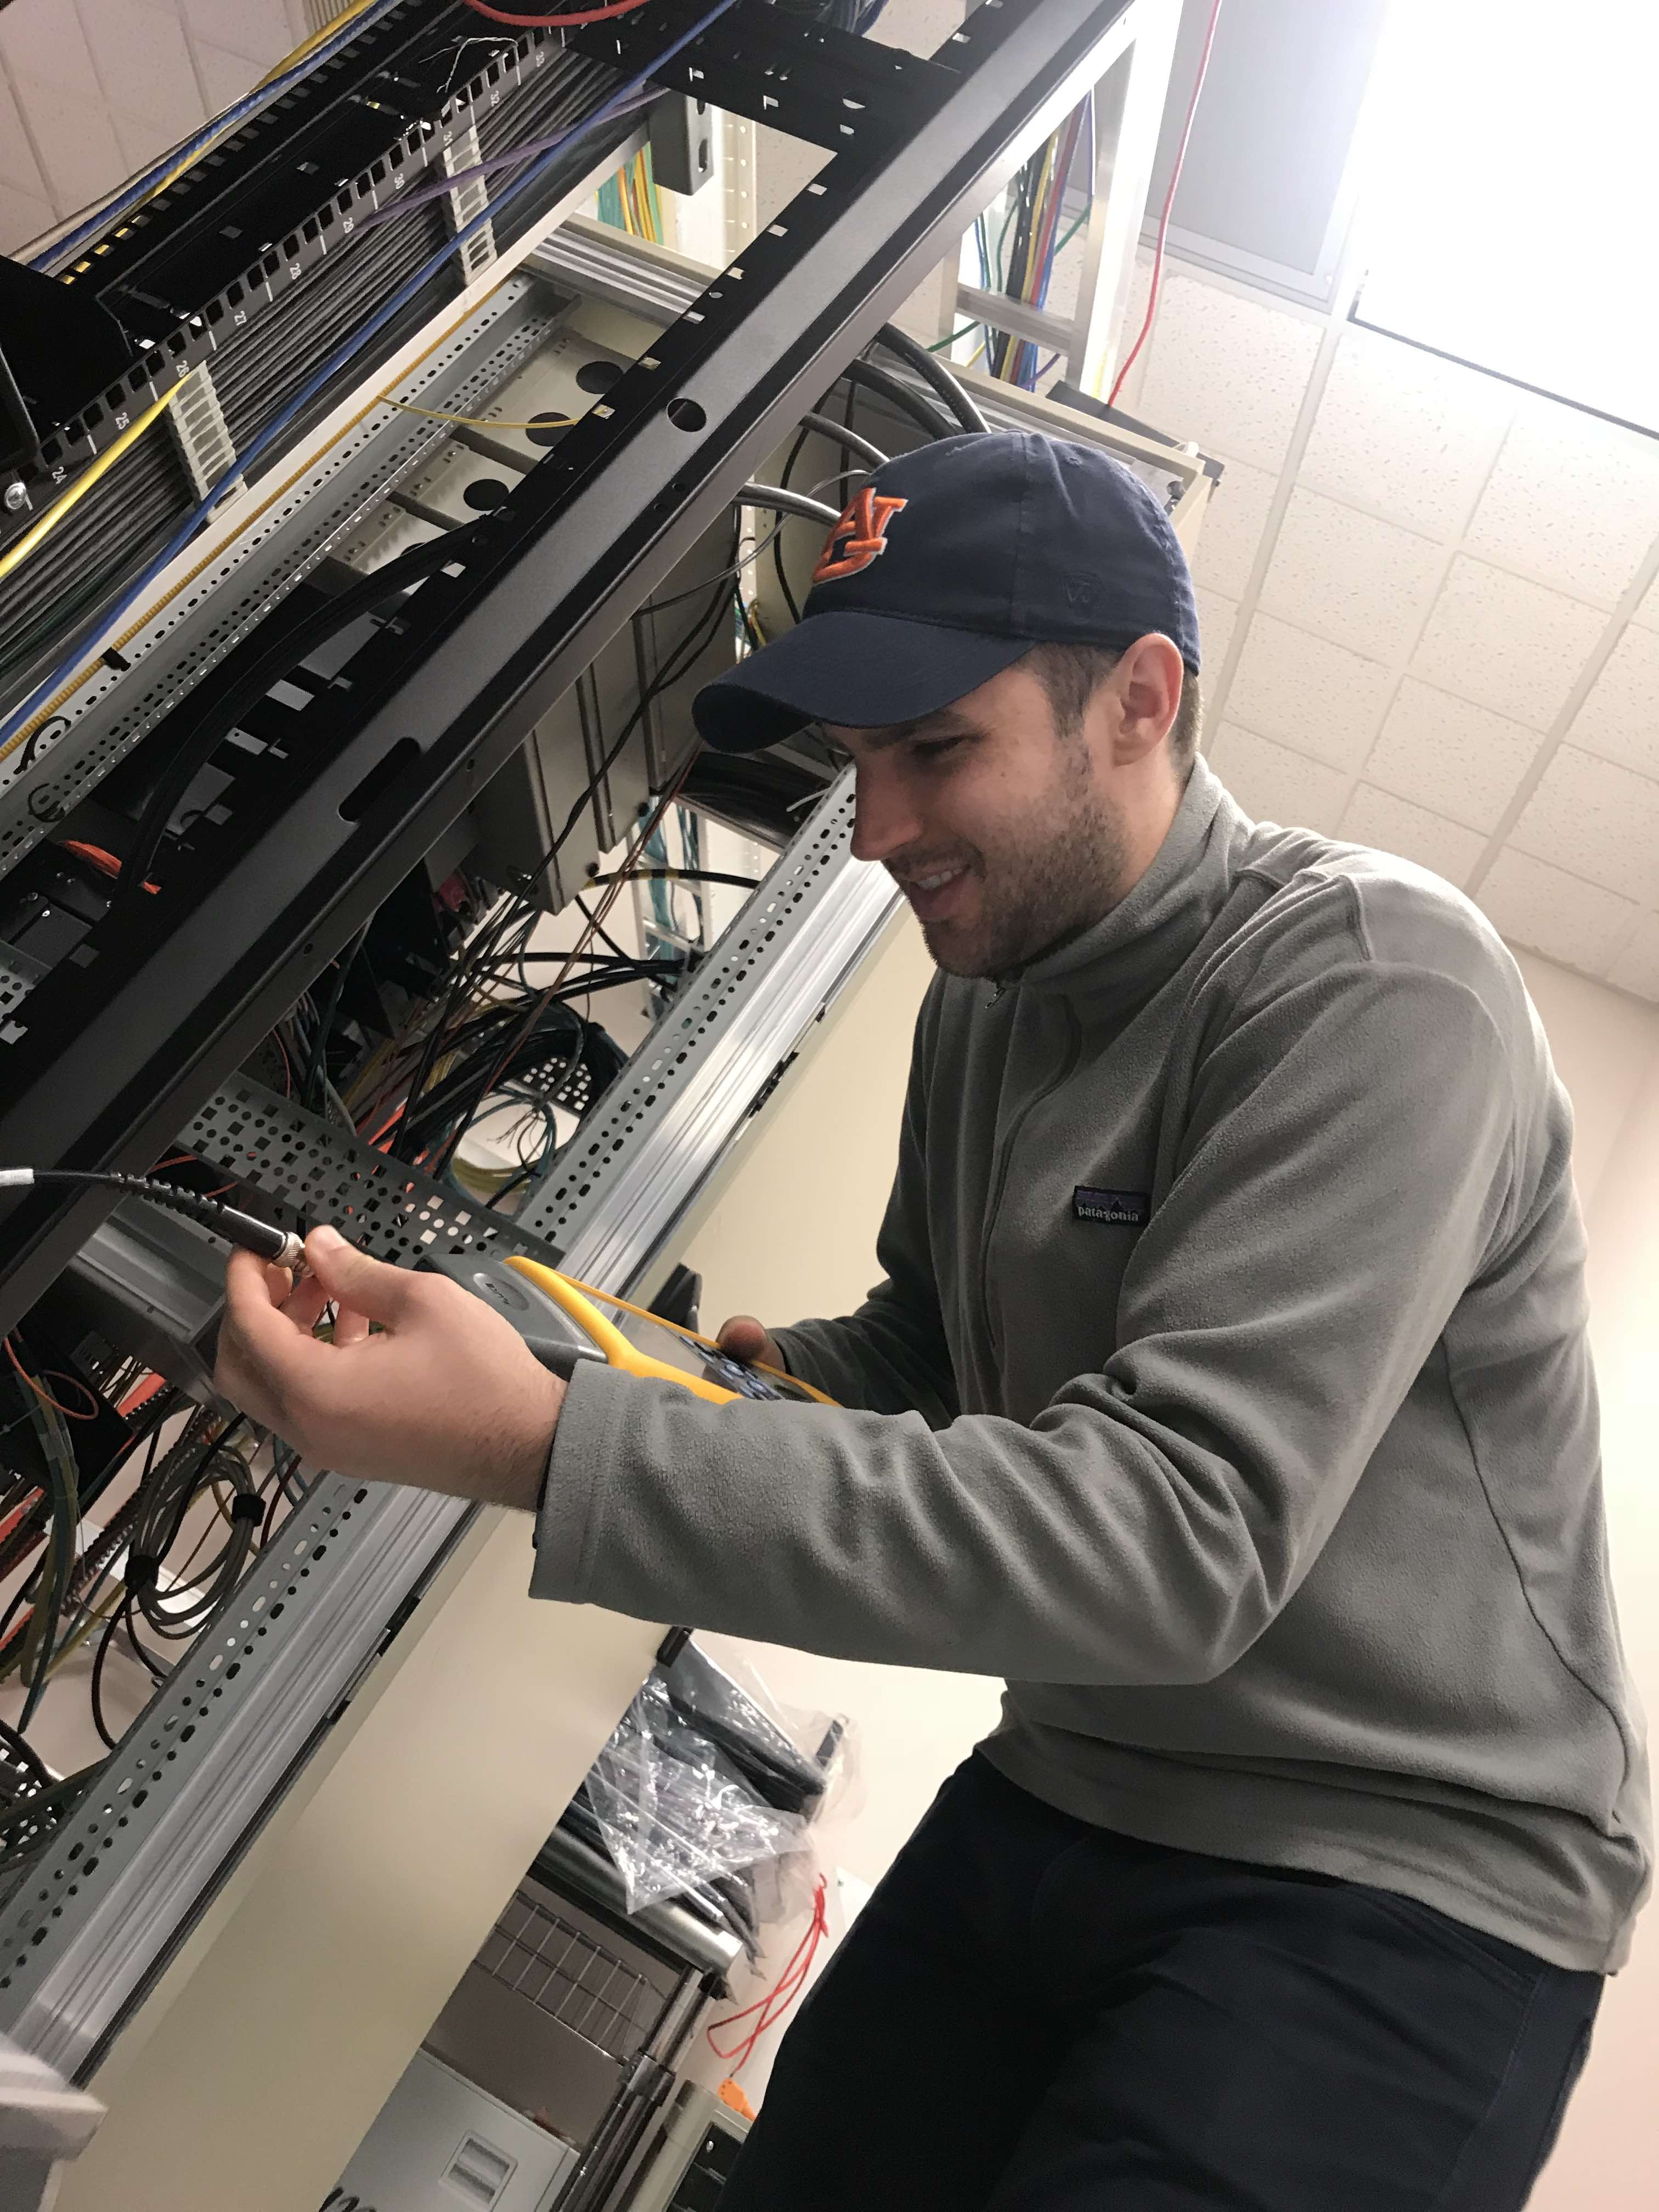
\includegraphics[width=0.8\linewidth]{img/rainer-performing-tdr.jpg}
	\end{center}
	\caption{Rainer Corley performing a Time Domain Reflectometry (TDR) cable length measurement on the cable running from the Symmetricom auxiliary GPS clock to the Timing Comparator (Aug. 2018).}
	\label{fig:rainertdr}
\end{figure}
\begin{figure}[!htb]
	\begin{center}
		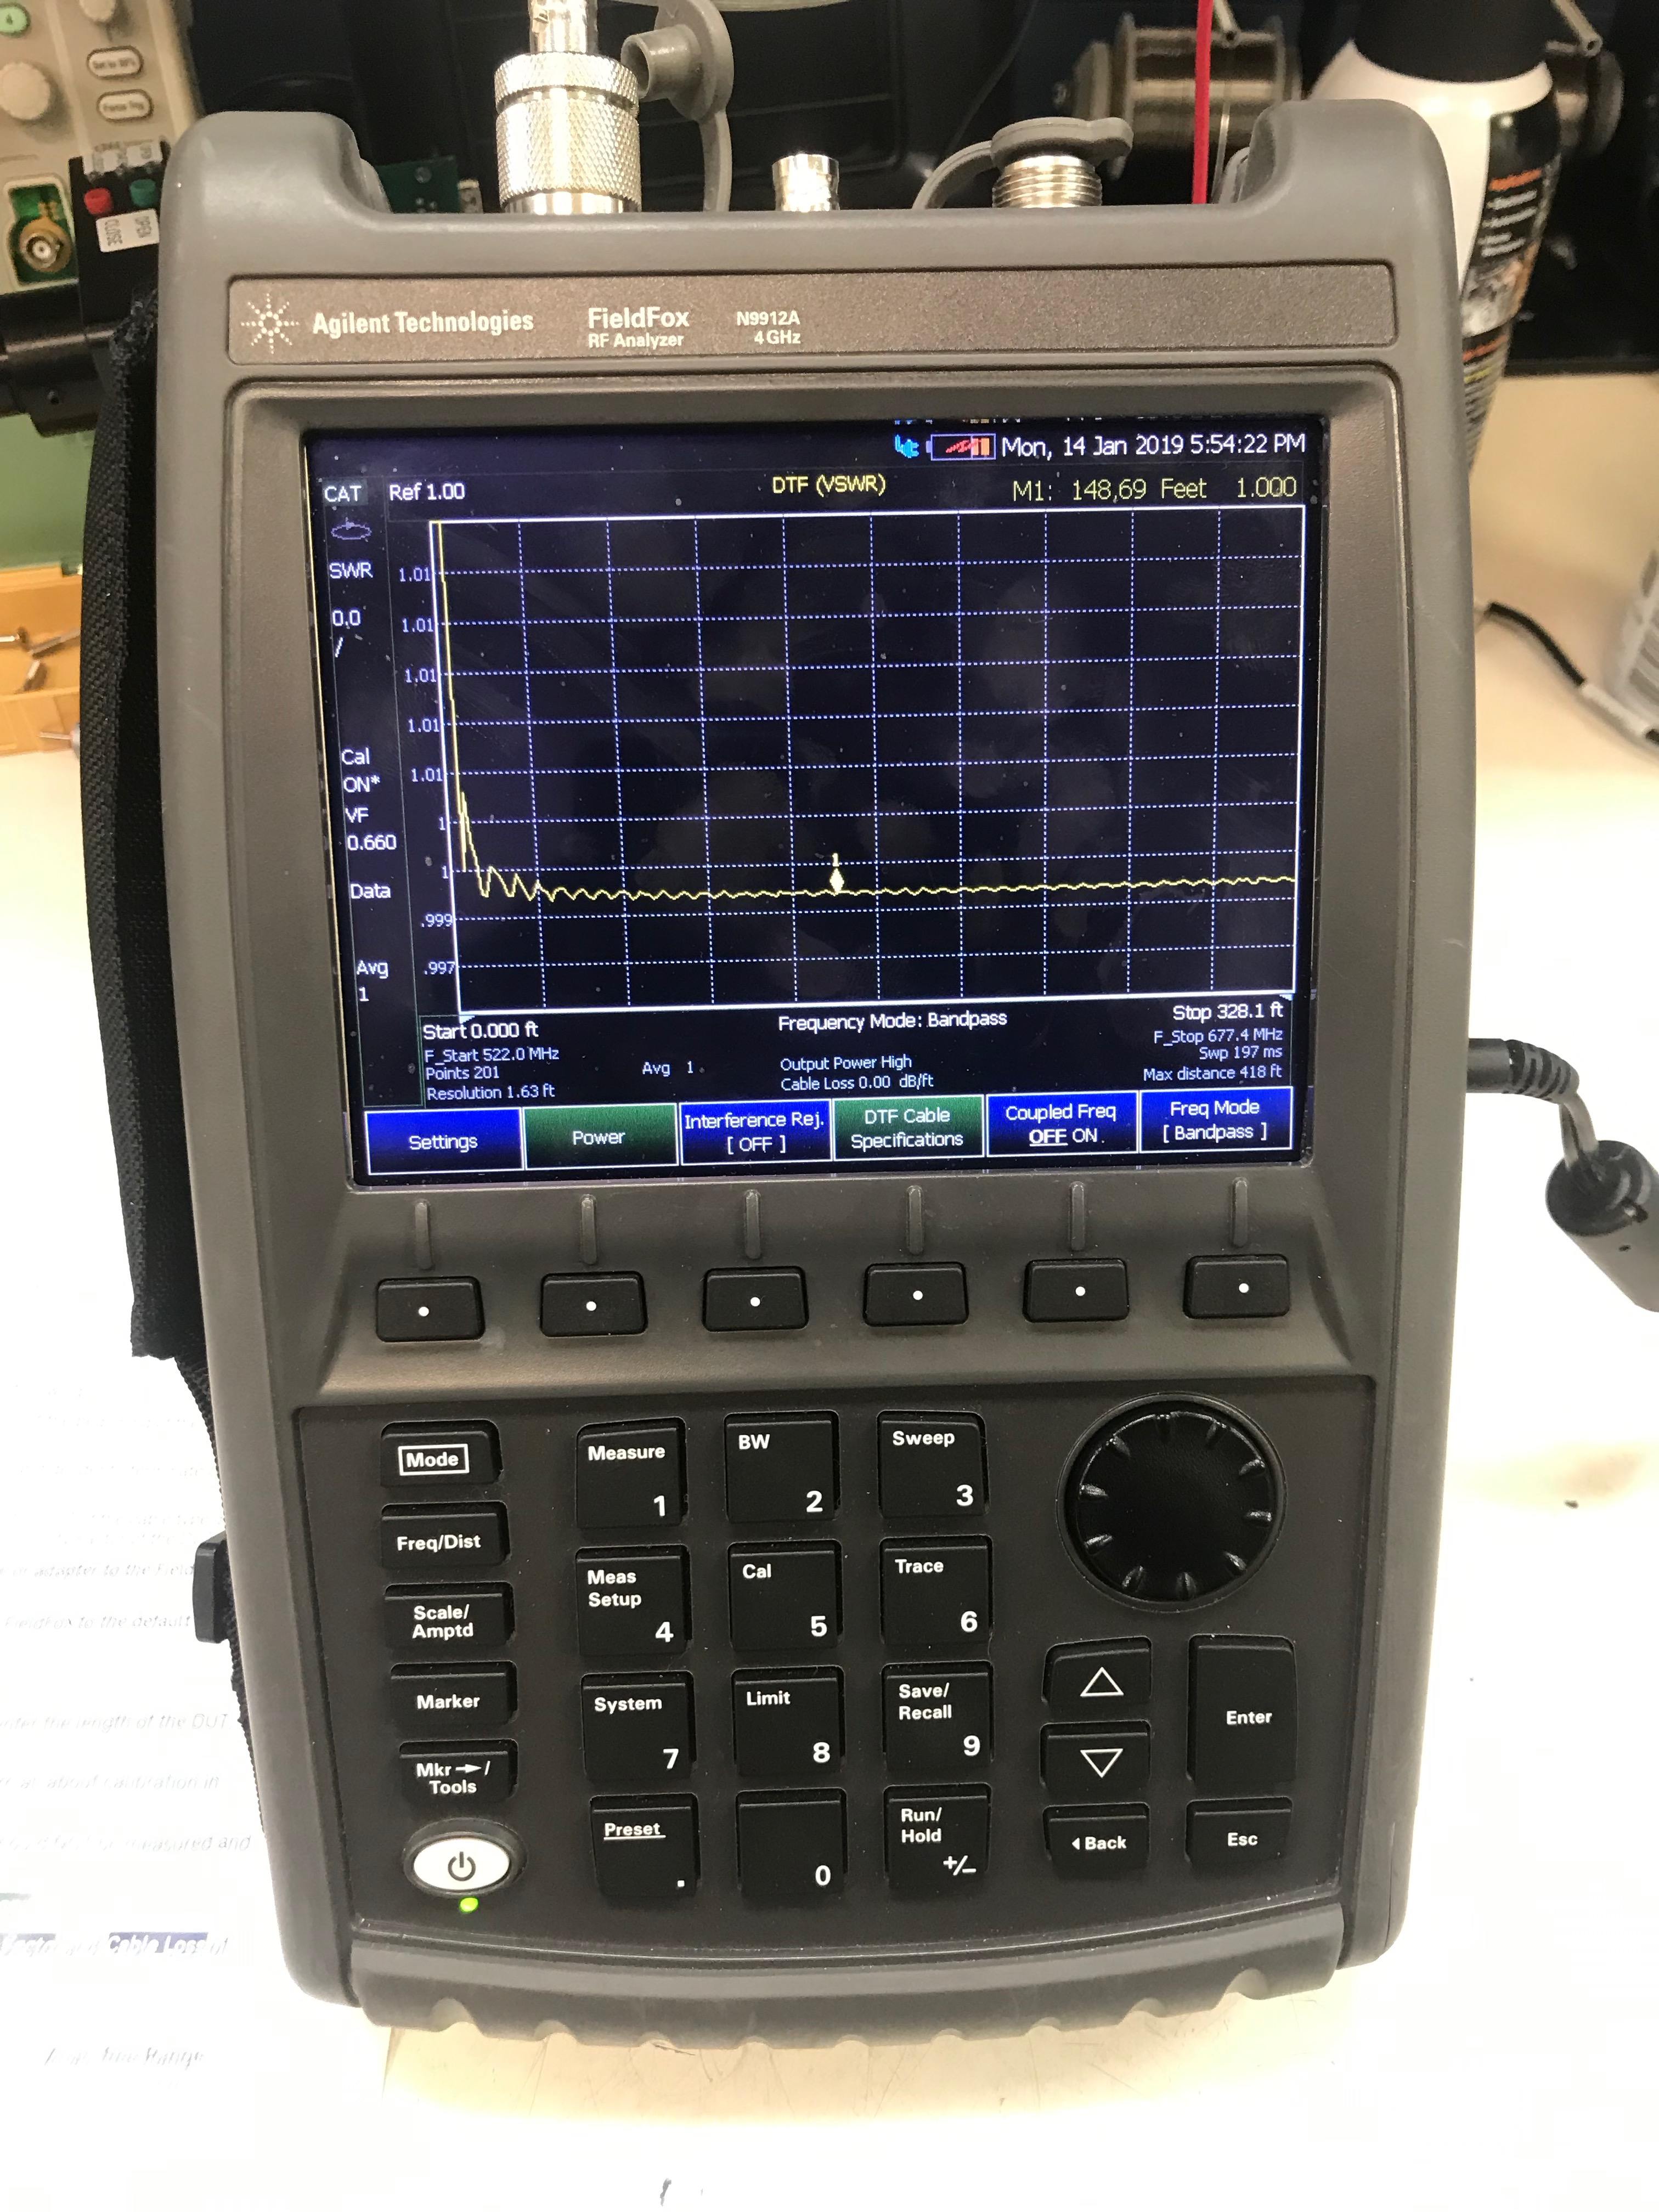
\includegraphics[width=0.8\linewidth]{img/time-domain-reflectrometer.jpg}
	\end{center}
	\caption{Device for performing \href{https://en.wikipedia.org/wiki/Time-domain_reflectometer}{Time Domain Reflectrometry} at LHO.}
	\label{fig:tdr-tool}
\end{figure}
\begin{figure}[!htb]
	\begin{center}
		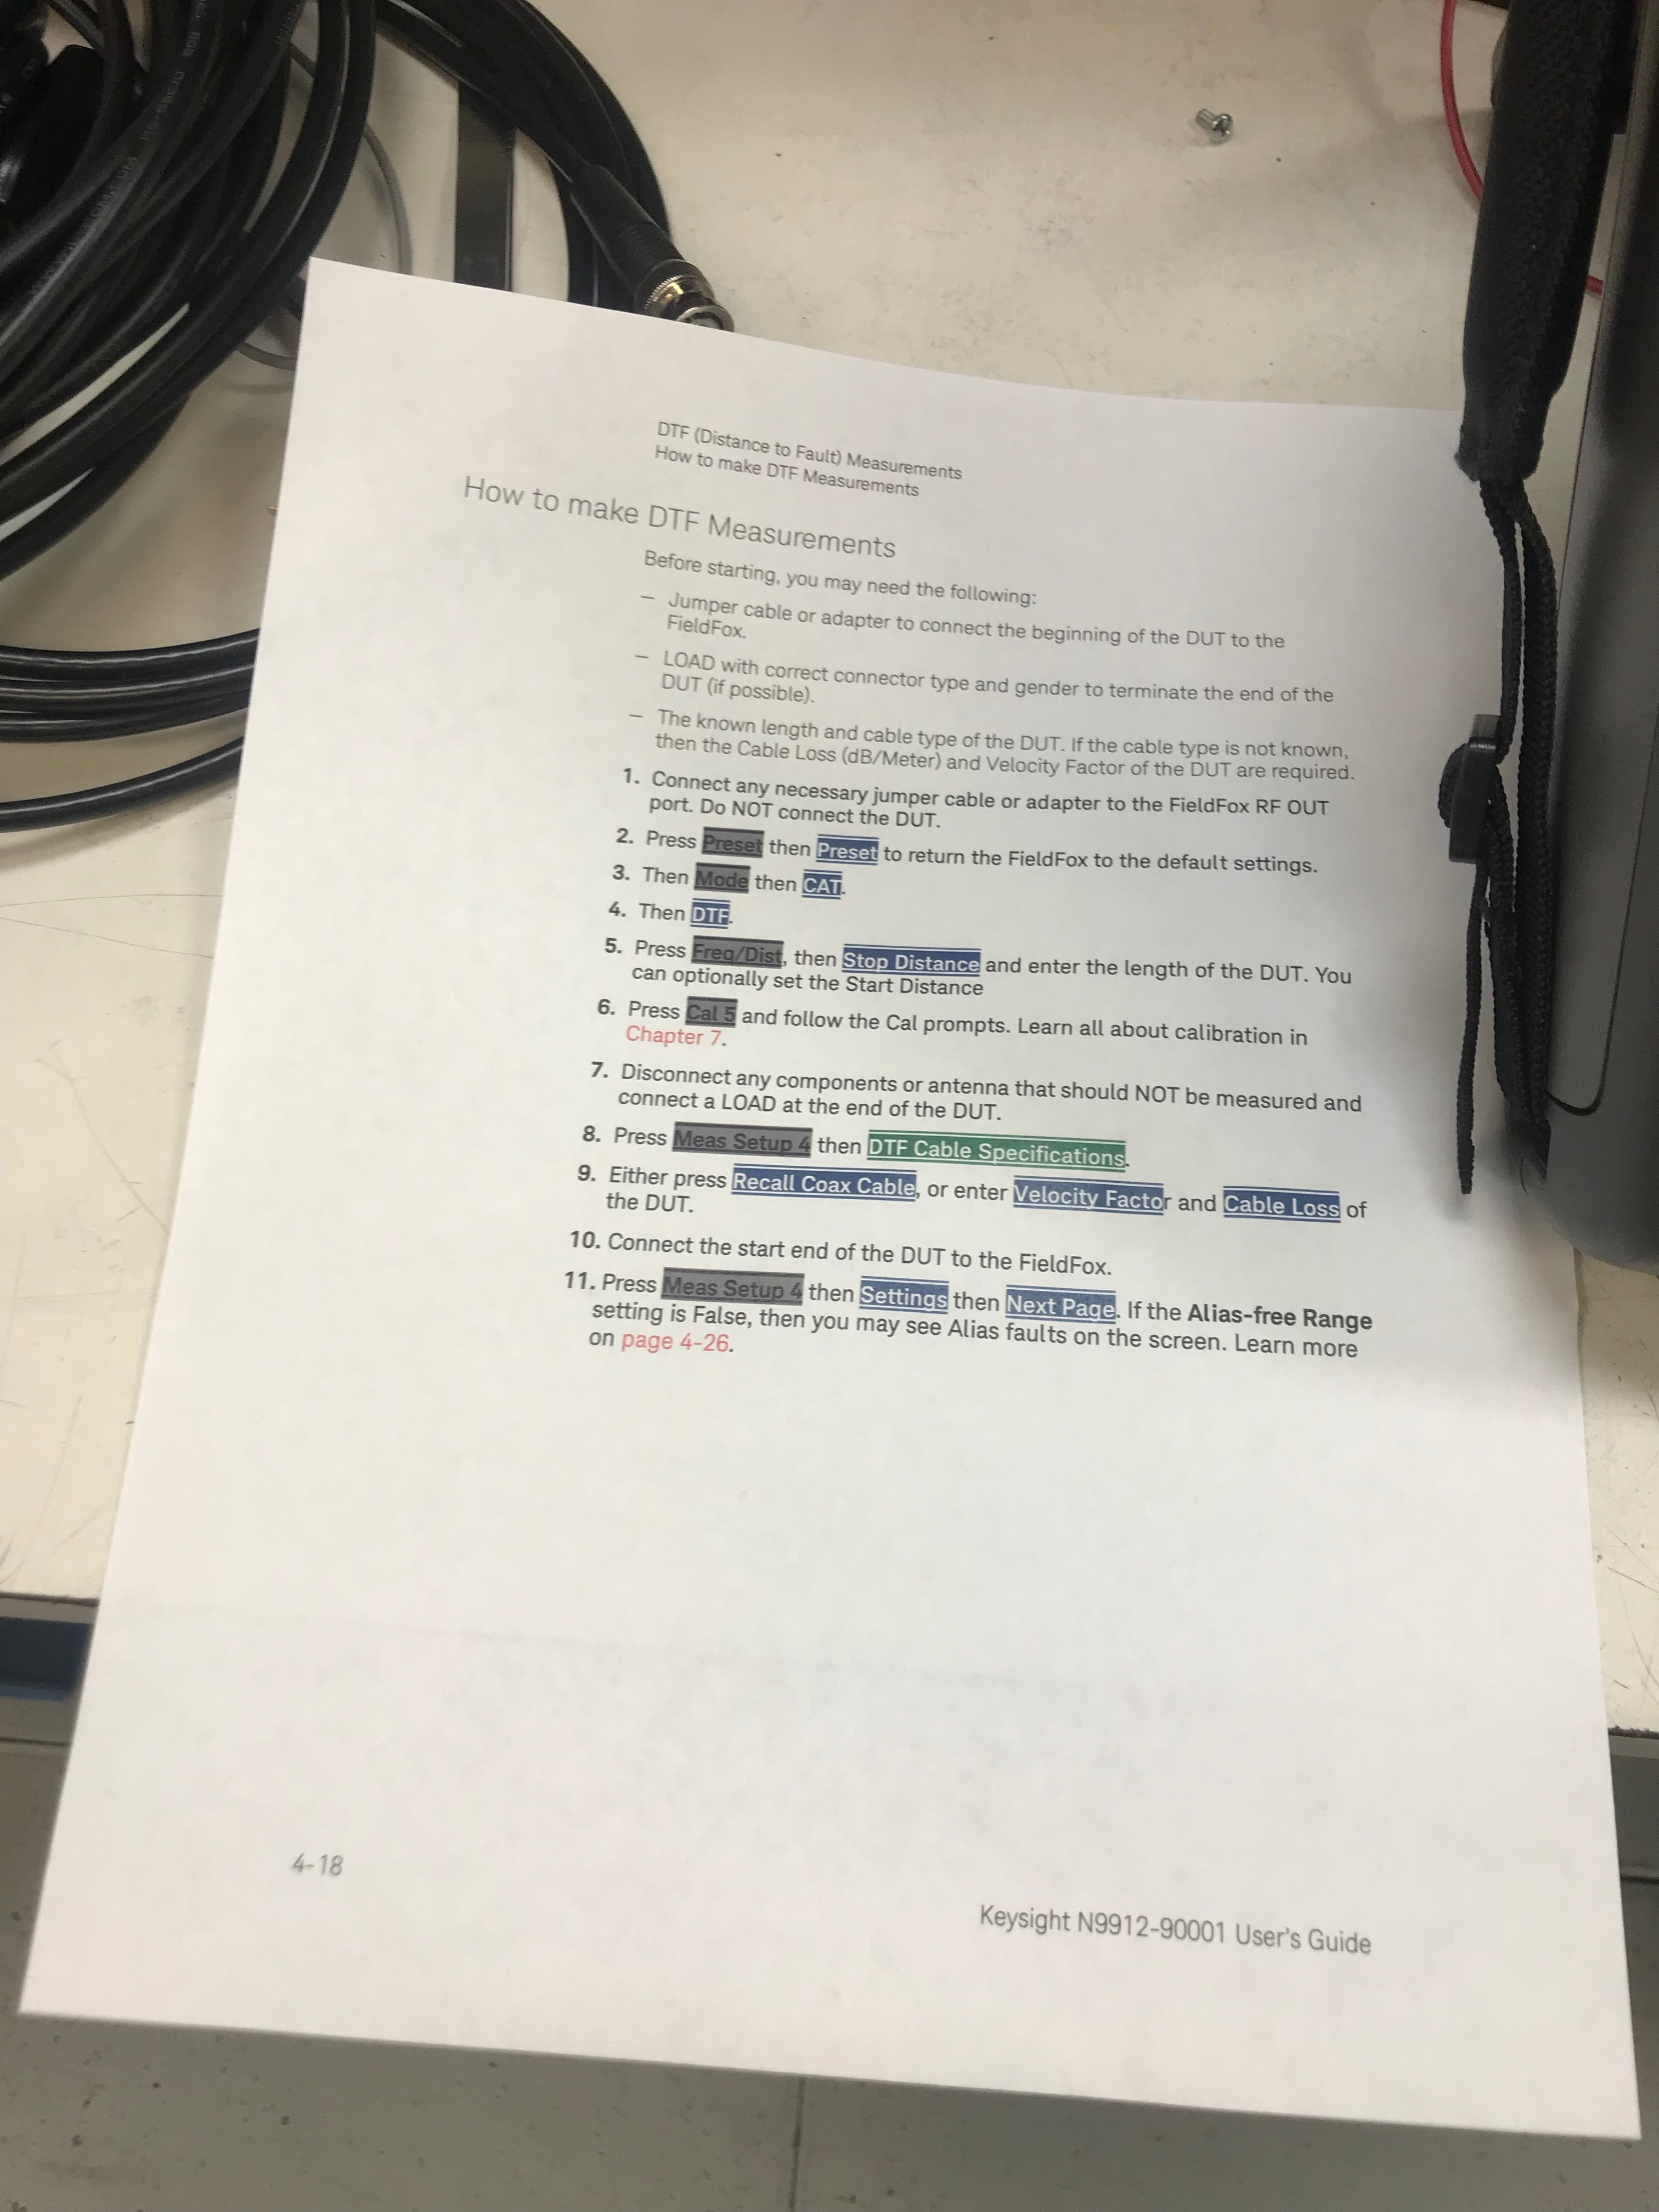
\includegraphics[width=0.8\linewidth]{img/time-domain-reflectrometer-dtf-instructions.jpg}
	\end{center}
	\caption{Instruction sheet for performing a DTF (Distance to Fault) distance measurement using this Time Domain Reflectrometer at LHO.}
	\label{fig:tdr-dtf-instructions}
\end{figure}
\begin{figure}[!htb]
	\begin{center}
		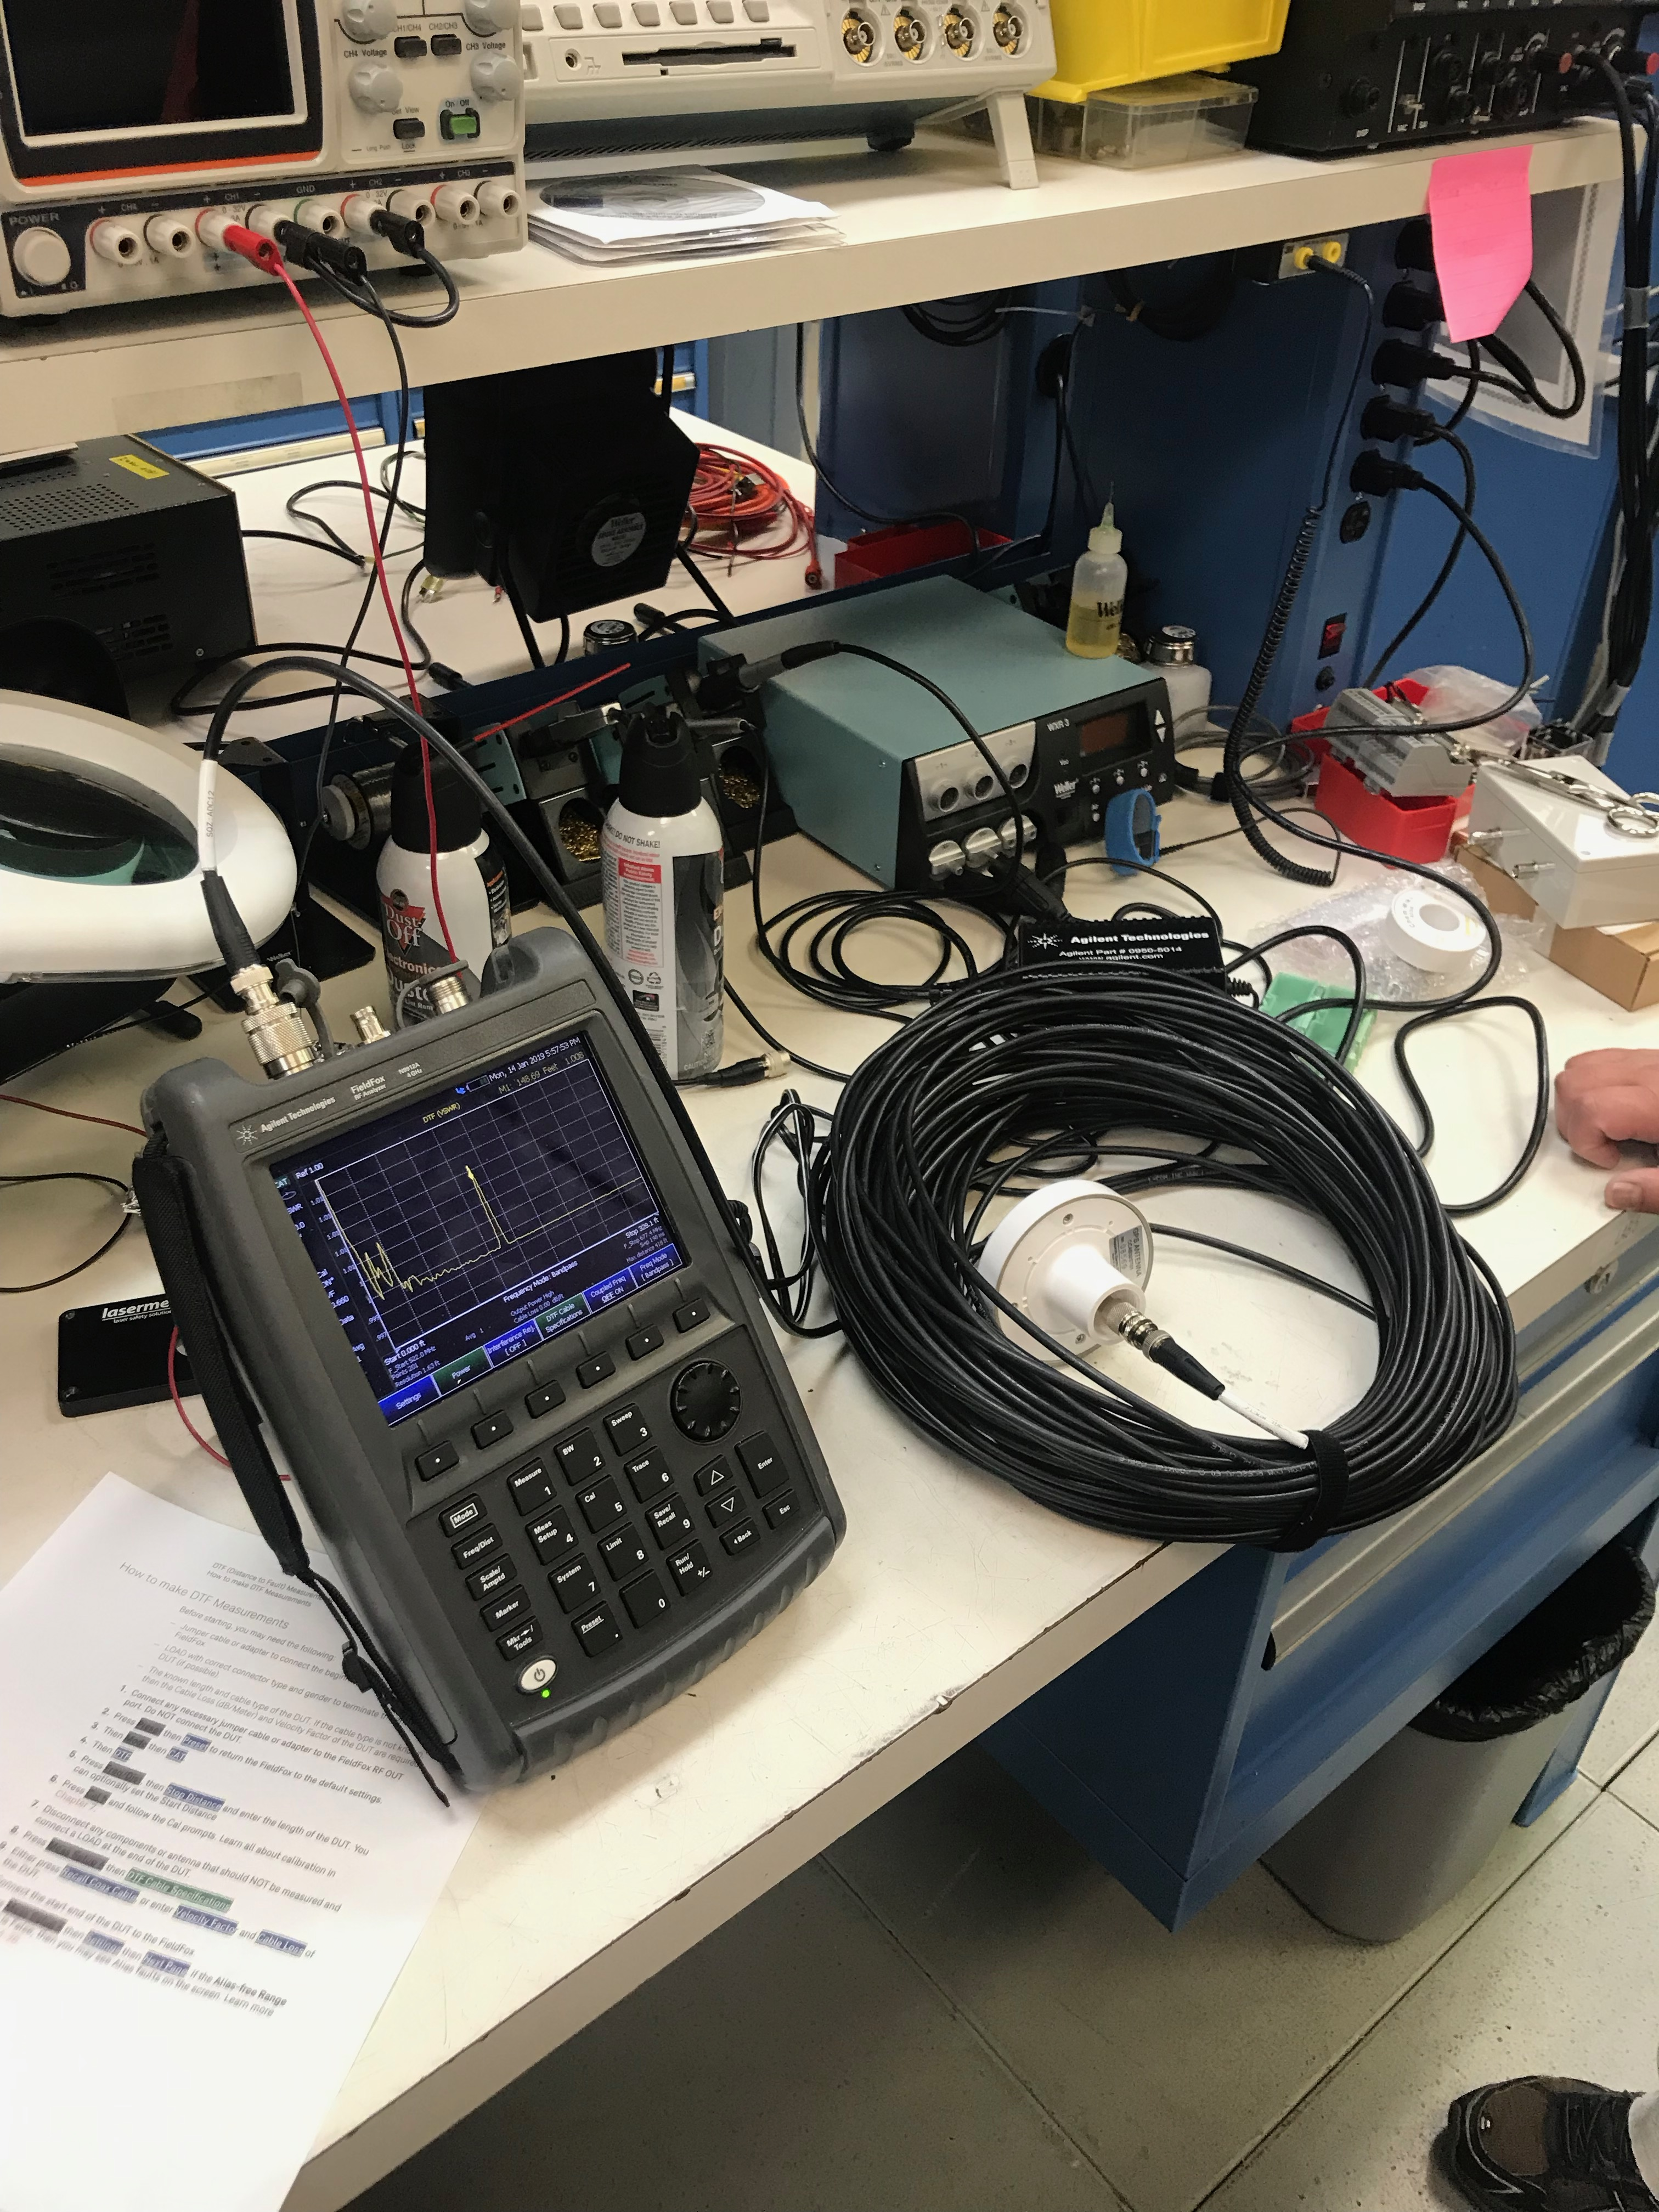
\includegraphics[width=0.8\linewidth]{img/time-domain-reflectrometer-dtf-test.jpg}
	\end{center}
	\caption{Proof of concept setup for measurement of a cable length terminated in a cable terminated by a GPS antenna.}
	\label{fig:tdr-test}
\end{figure}
\begin{figure}
	\begin{center}
		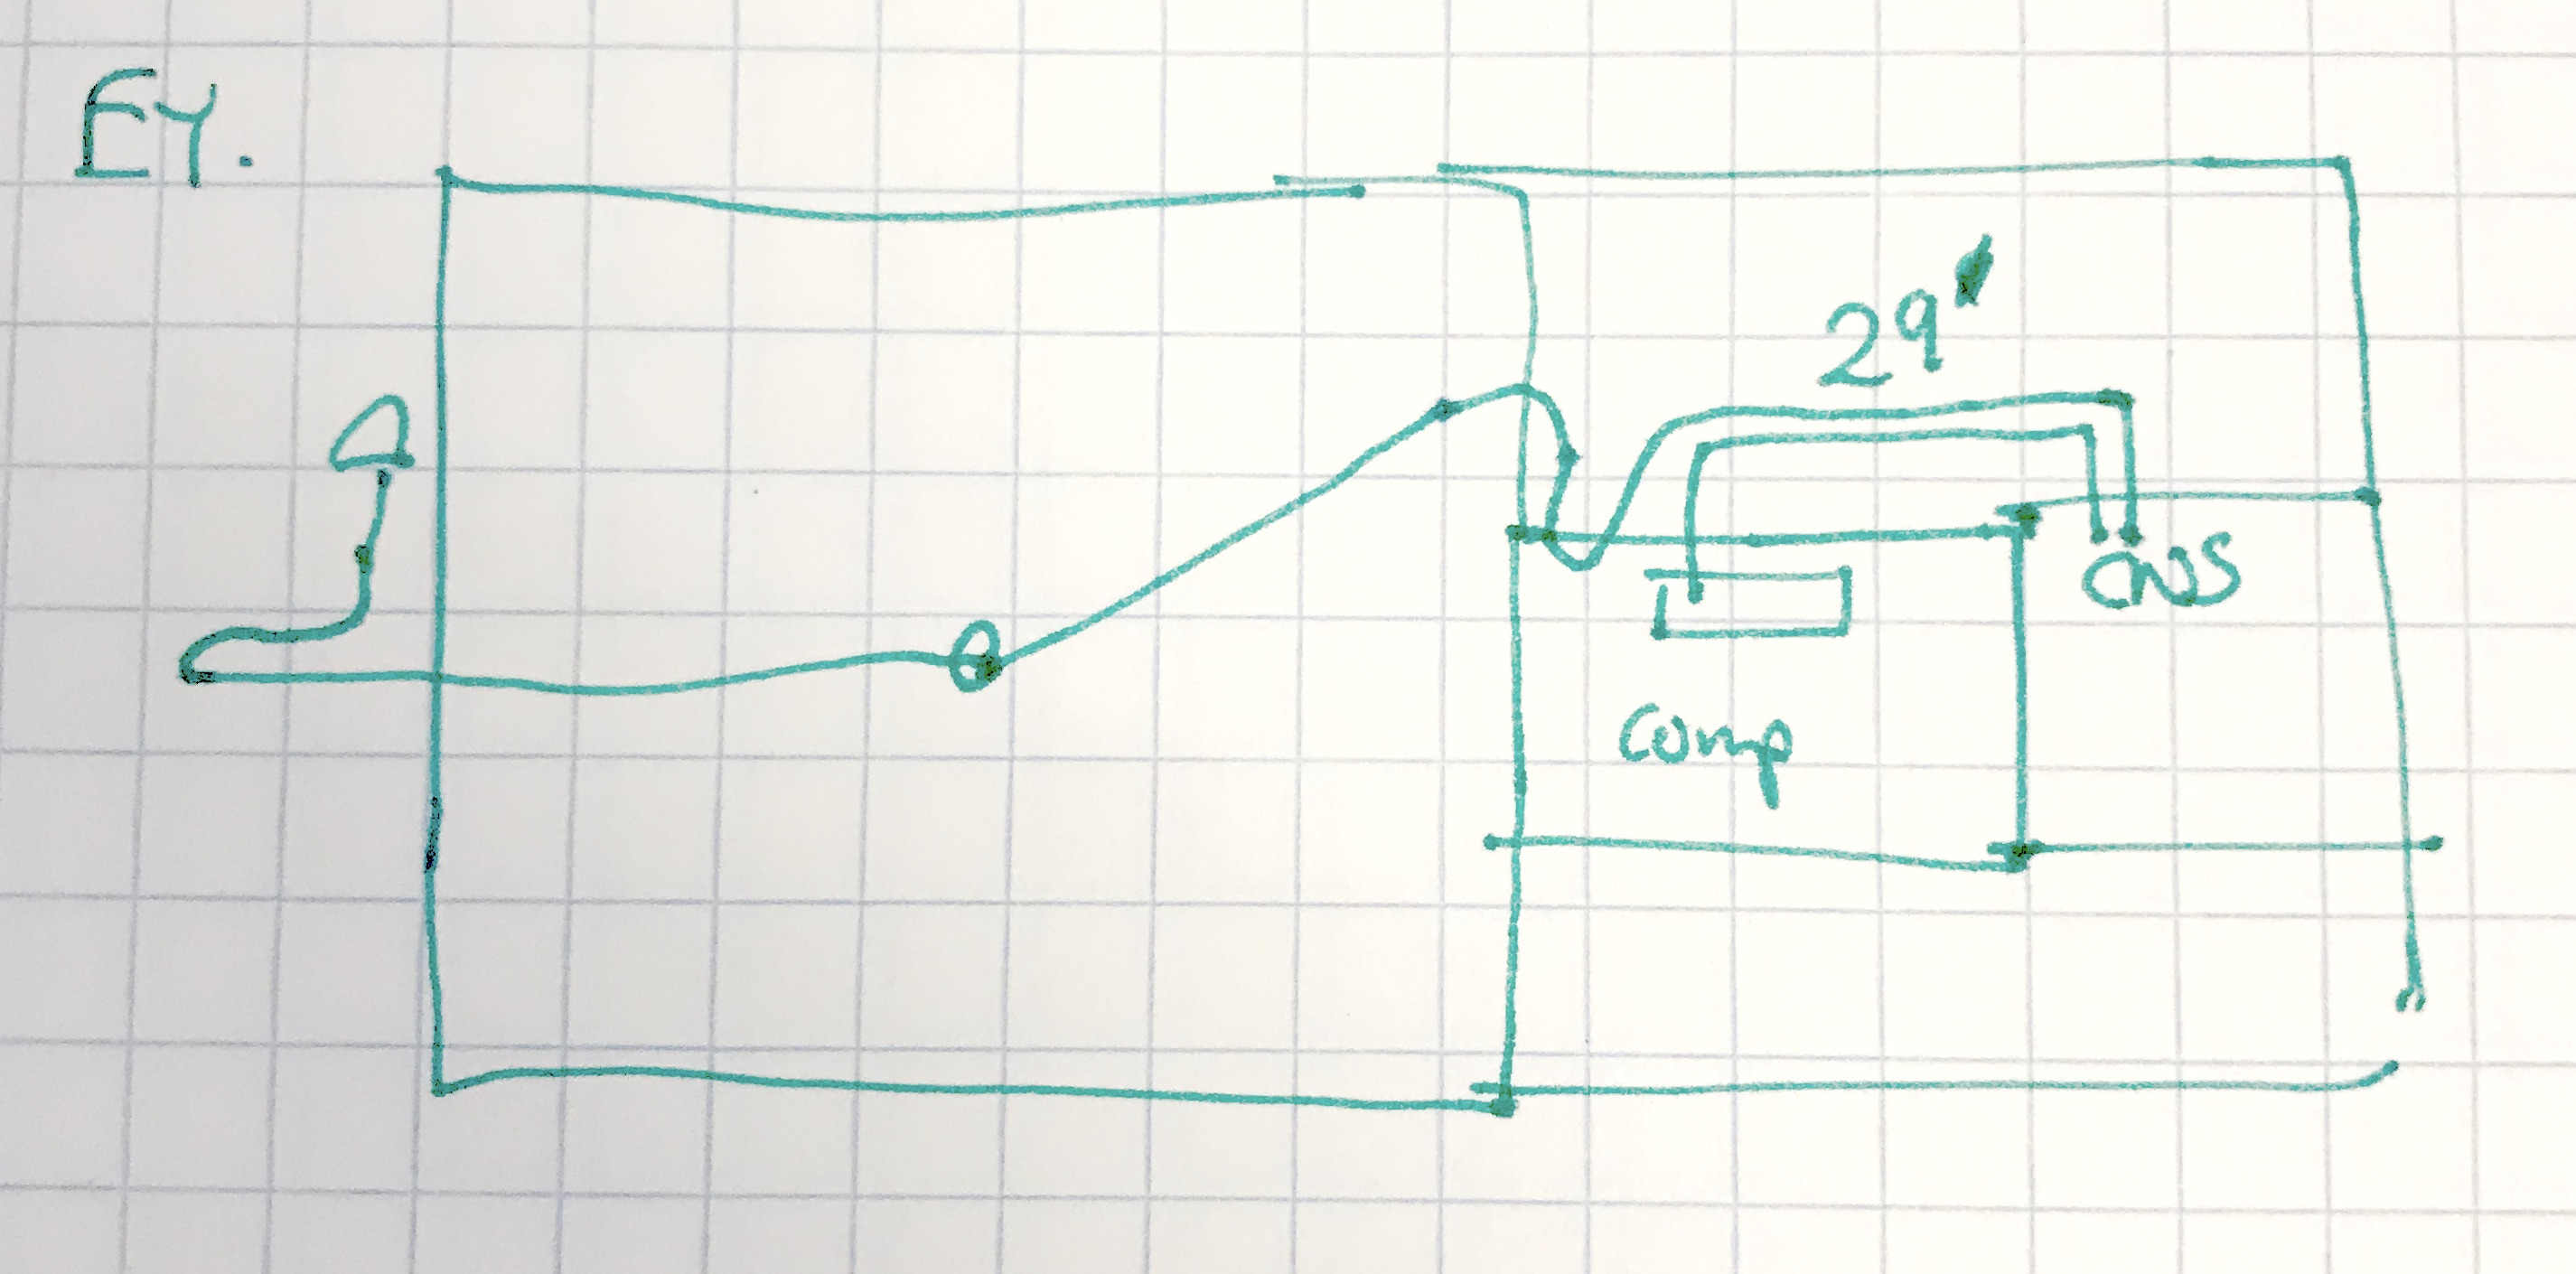
\includegraphics[width=0.8\linewidth]{img/endstation-antenna-cable.jpeg}
	\end{center}
	\caption{Cartoon by Dave Barker of CNS II GPS cable routing from clock to antenna in end stations. We can ask Dave for a more precise diagram/description if we really care about thse lengths.}
	\label{fig:routing}
\end{figure}
\begin{figure}
  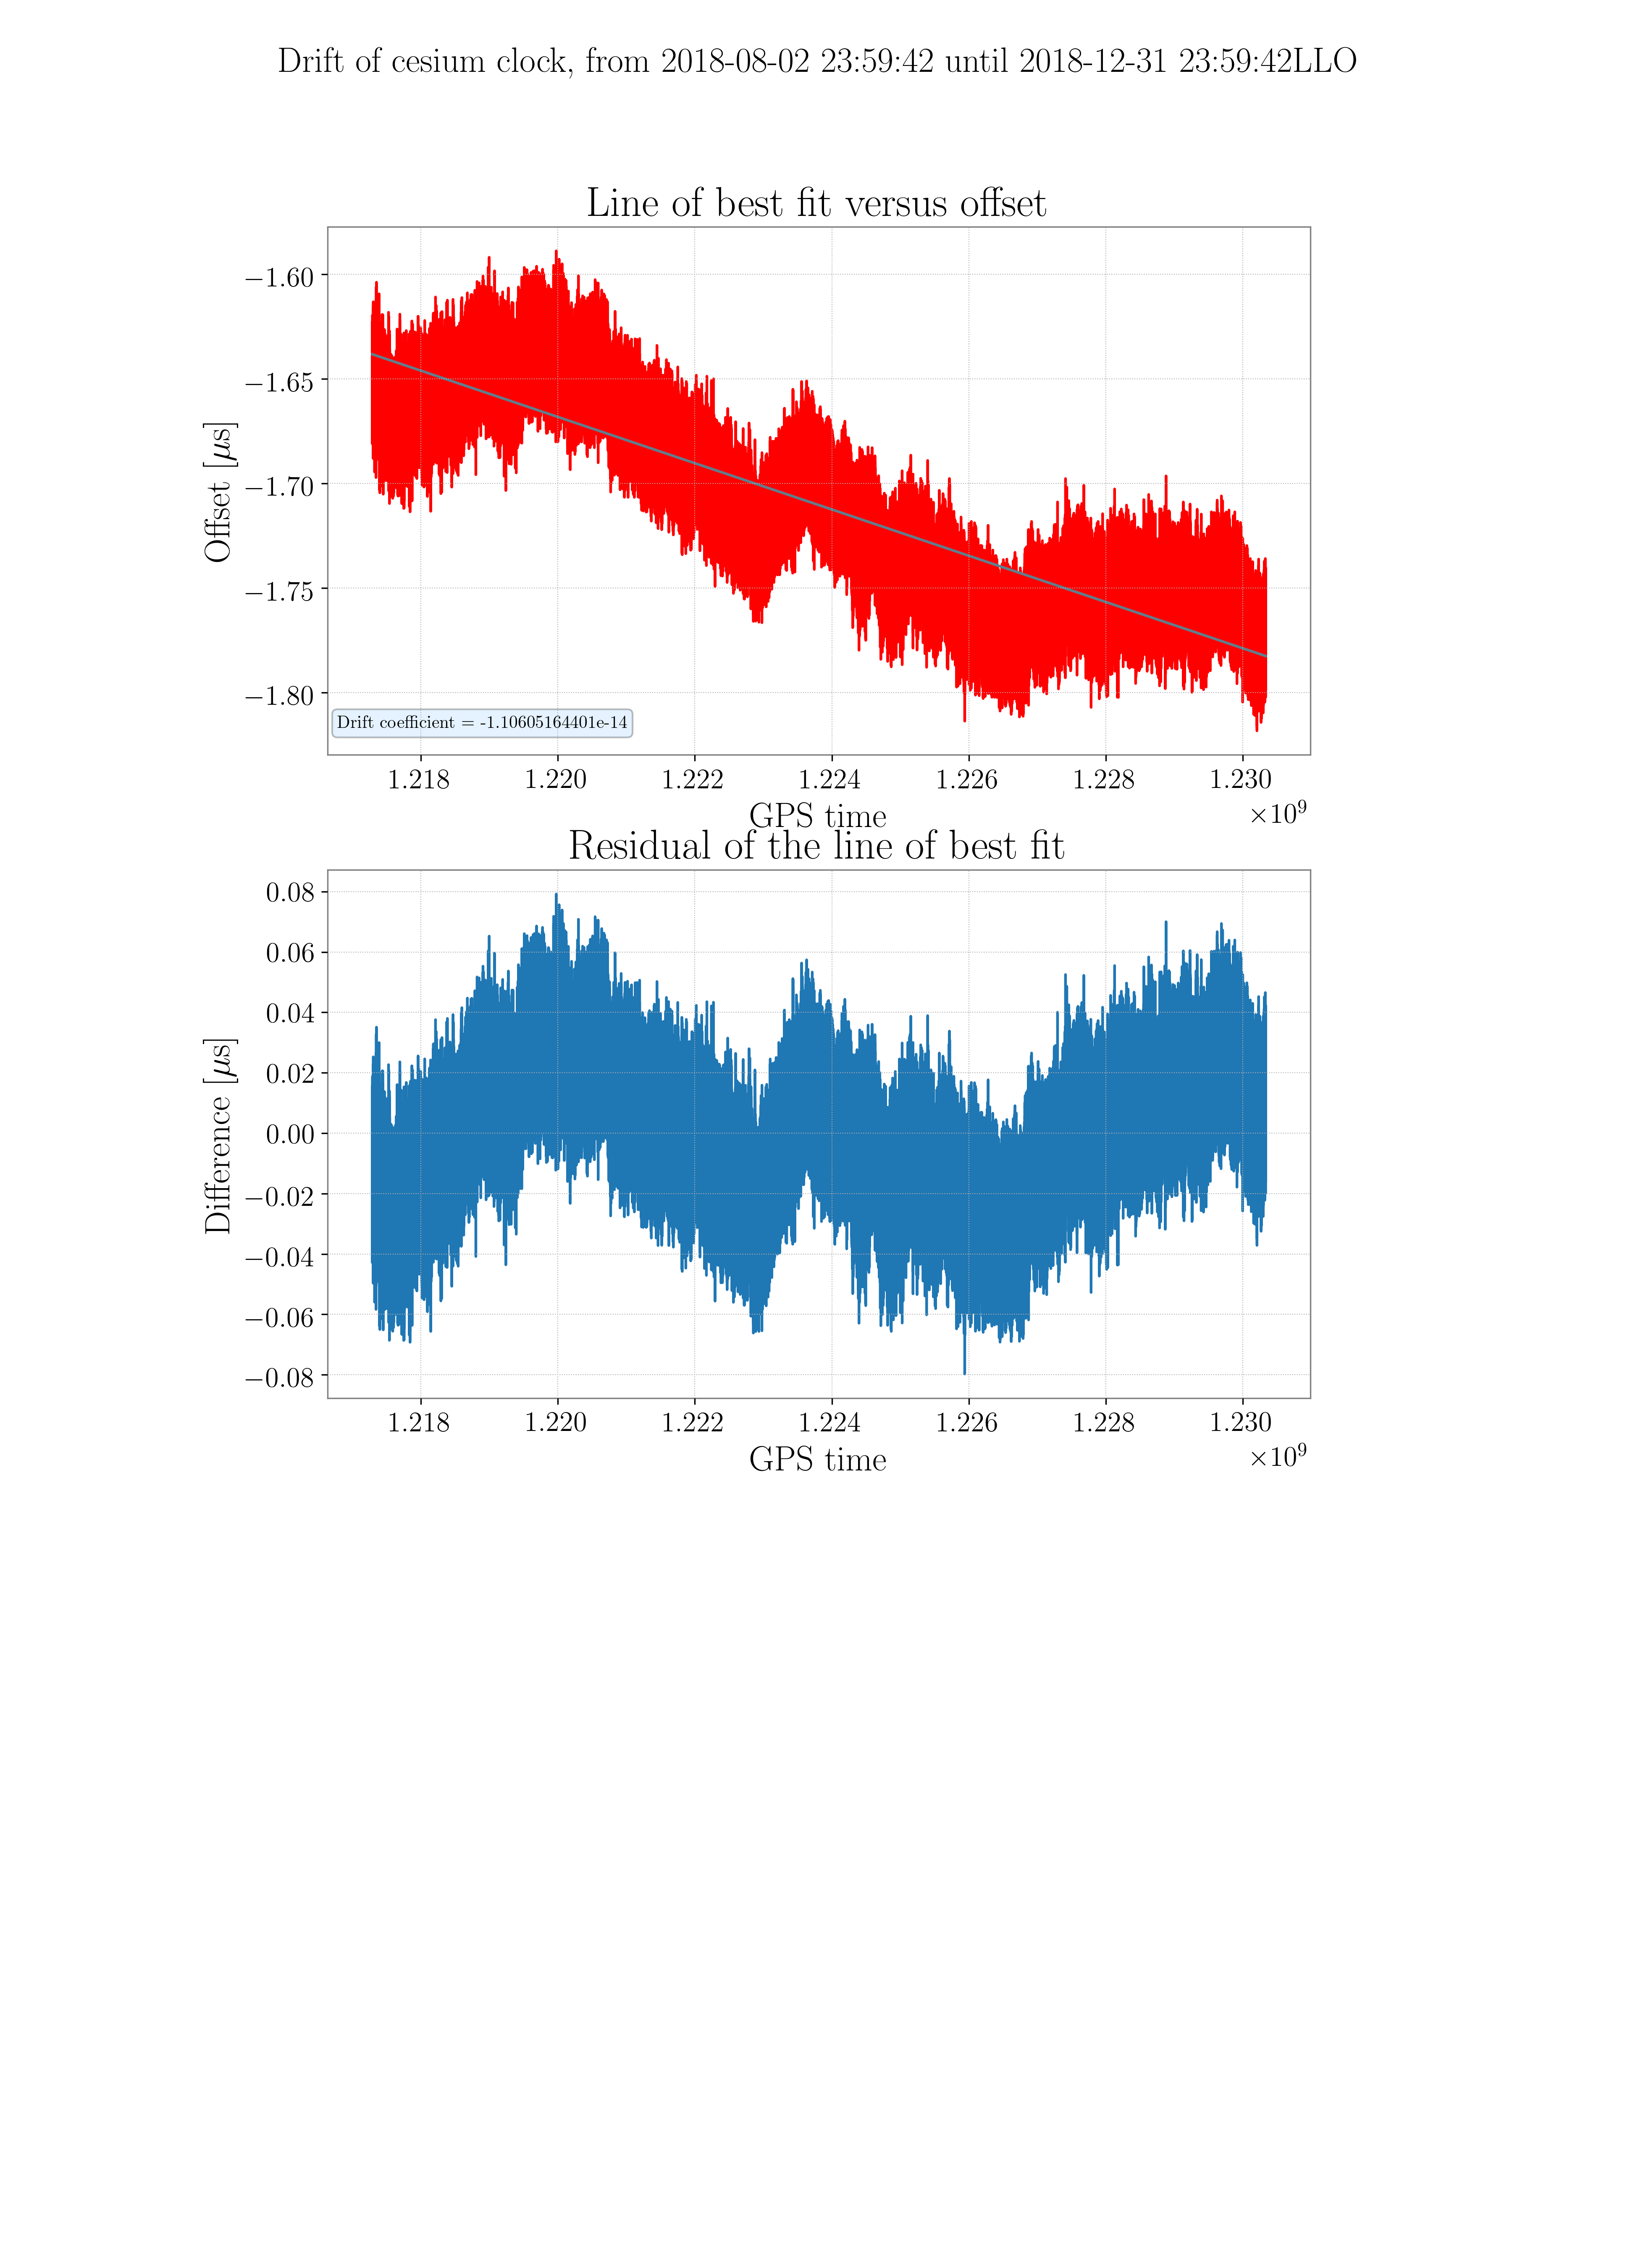
\includegraphics[width=\linewidth]{img/cesium-clock.png}
  \caption{Cesium 1PPS clock time difference vs. Timing System over last few months. Differences should resemble a linear trend with deviations on the order of hundreds of nanoseconds; the above result demonstrates a clear failure of the Time Code Generator (TCG) used in aLIGO's timing diagnostic system.}
  \label{fig:cesium}
\end{figure}
\clearpage

\section{LLO Cable Lengths}
\label{sec:llocables}
\begin{center}
  \begin{tabular}{ | l | l | l | l | }
    \hline
    \textbf{Cable Name}                 & \textbf{Type} & \textbf{Length (ft)}  & \textbf{Description} \\ \hline
    L1:TIM-EY\_GPS\_1PPS                & RG-58         & 18                    & Y-End CNS II 1PPS \\ \hline
    L1:TIM-EX\_GPS\_1PPS                & RG-58         & 20                    & X-End CNS II 1PPS \\ \hline
    L1:TIM-CSIII\_1PPS                  & RG-58         & 4                     & Cs-III 1PPS to rack plate \\ \hline
    1PPS GPS NTS                        & RG-58         & 3                     & NTP Server 1PPS to rack plate \\ \hline
    (No name)                           & RG-58         & 2                     & Rack plate Cs-III 1PPS to Comp. \\ \hline
    CAB\_L1:ACT-TTPPS\_012 (Repurposed) & RG-58         & 2                     & Rack plate NTP 1PPS to Comparator \\ \hline
                                        & LMR-400       & 0                     & Timing Master GPS Antenna Cable \\ \hline
    TRIMBLE ANTENNA                     & LMR-400       & 0                     & Trimble GPS Antenna Cable \\ \hline
    GPS ANT                             & LMR-195       & 0                     & Y-End CNS II GPS Antenna Cable \\ \hline
    GPS ANT                             & LMR-195       & 0                     & X-End CNS II GPS Antenna Cable \\ \hline
    H1:DAQ (Repurposed)                 & RG-58         & 1                     & Trimble to Master 1PPS cable \\ \hline
    (No name)                           & RG-58         & 2                     & 58539A Lightning arrestor to Trimble \\ \hline
    (No name)                           & RG-58         & 3                     & 58539A Lightning arrestor to Master \\ \hline
  \end{tabular}
\end{center}
\clearpage

\end{document}
